\documentclass{article}
\usepackage{graphicx}
\usepackage{titling}
\usepackage{hyperref}

\begin{document}

% First page
\begin{titlepage}
    \vspace*{\fill}
    \begin{center}
        \Large \textbf{Project report} \\
        \vspace{0.5cm}
        \rule{\textwidth}{1pt} \\
        \vspace{0.5cm}
        \Huge \textbf{Bitcoin prediction model} \\
        \vspace{0.5cm}
        \rule{\textwidth}{1pt} \\
        \vspace{1cm}
        \Large Chantoiseau Sacha\\Cherigui Allah Eddine\\Louis Malmassary\\
        \vspace{1cm}
        \normalsize \today
    \end{center}
    \vspace*{\fill}
    \begin{flushleft}
        
\includegraphics[width=0.2\textwidth]{img/UCA.png}
    \end{flushleft}
\end{titlepage}

\newpage

\tableofcontents

\newpage

\section{Introduction}
The goal of this project is to develop a predictive model for Bitcoin prices using machine learning techniques. Bitcoin, being a highly volatile cryptocurrency, presents a challenging task for accurate price prediction. The primary objective is to build a model that can predict future Bitcoin prices based on historical data, thereby providing insights and aiding in decision-making for investors and traders.

\section{Data Set Description}
The data set used for this project consists of historical Bitcoin prices obtained from a publicly available source. The data includes daily prices of Bitcoin in USD, along with other relevant features such as the date. The data preprocessing steps involved the following:
\begin{itemize}
    \item Reading the raw data from a CSV file.
    \item Converting the date column to a datetime format.
    \item Extracting additional features such as year and month from the date.
    \item Normalizing the relevant columns to ensure that the data is on a similar scale.
    \item Aggregating the data on a monthly basis to reduce noise and capture long-term trends.
\end{itemize}
The preprocessed data is then saved to a new CSV file for further analysis and model training.

\section{Methodology}
The methodology followed in this project involves several key steps:
\subsection{Model Selection}
Given the time series nature of the data, an LSTM (Long Short-Term Memory) neural network was chosen for the prediction task. LSTM models are well-suited for time series data as they can capture temporal dependencies and patterns.
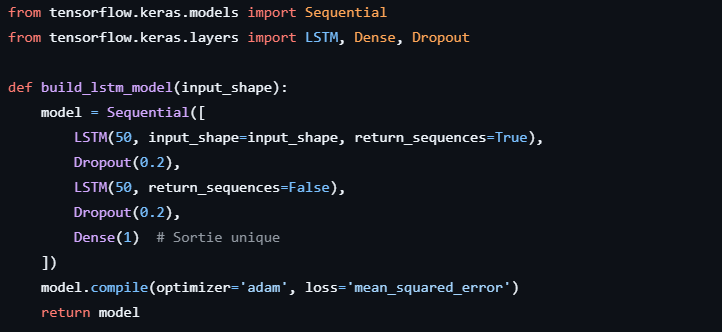
\includegraphics[width=0.8\textwidth]{img/model}

\subsection{Data Preparation}
The preprocessed data is divided into time windows to create input sequences for the LSTM model. Each time window consists of a fixed number of past observations used to predict the next value in the sequence. The data is then split into training and testing sets to evaluate the model's performance.

We use the loadAndPreprocessData function to load a CSV file, process the date column to extract the year and month, normalize specific financial columns with MinMaxScaler, and group the data by year and month, calculating the mean for each group. It returns the monthly aggregated data with normalized values, indexed by date.

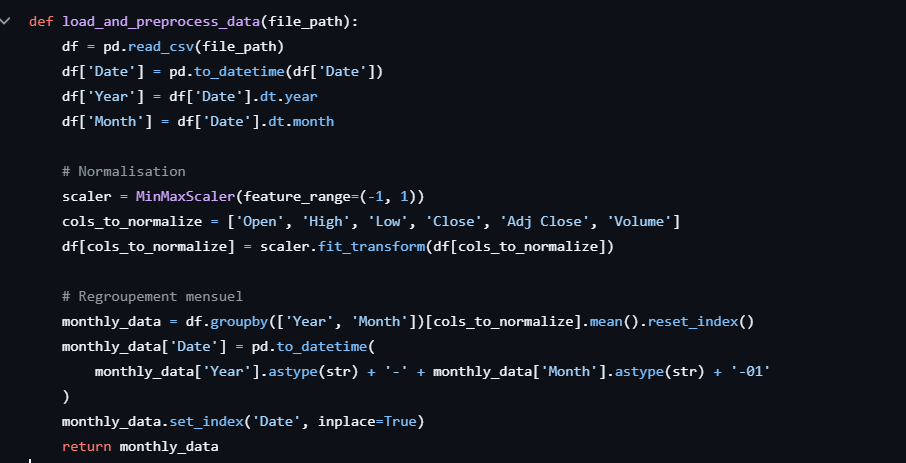
\includegraphics[width=0.8\textwidth]{img/Capture d’écran 2025-01-05 200052.png}
\subsection{Model Training}
The LSTM model is built using the Keras library with TensorFlow as the backend. The model consists of two LSTM layers and two Dropout layers to prevent overfitting. The model is compiled with the Adam optimizer and mean squared error loss function. The training process involves fitting the model to the training data and saving the trained model and test data for evaluation.

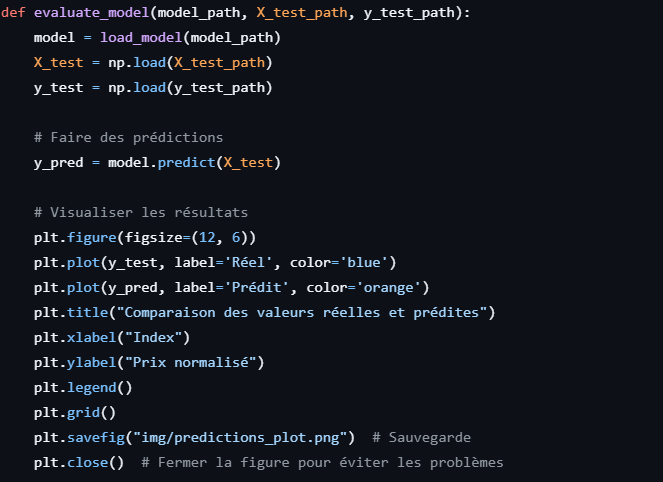
\includegraphics[width=0.8\textwidth]{img/evaluation.png}
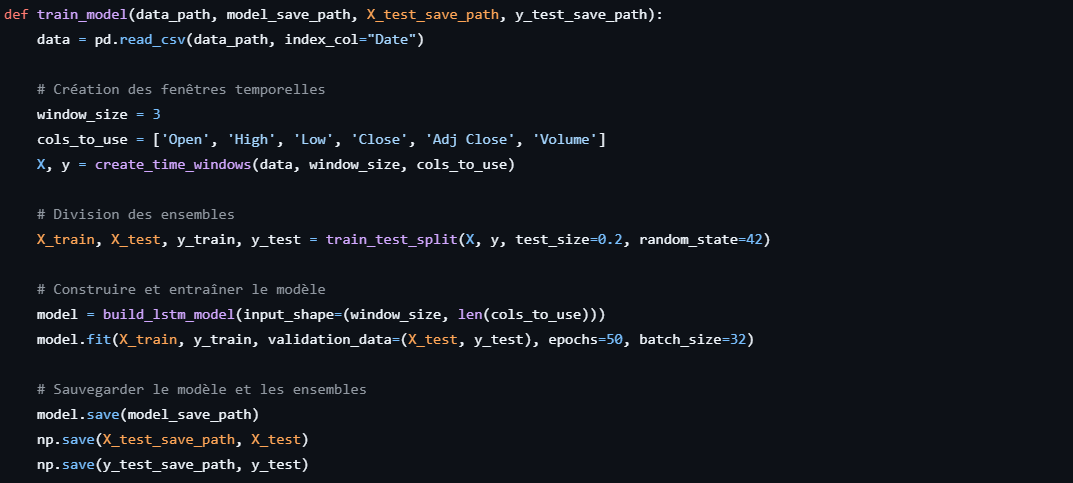
\includegraphics[width=0.8\textwidth]{img/Capture d’écran 2025-01-05 201711.png}

\section{Results}
\subsection{Model Performance}
The performance of the model was evaluated using the test data. The primary metric used for evaluation was the mean squared error (MSE) between the predicted and actual Bitcoin prices. The results indicate that the model was able to capture the general trend of Bitcoin prices, although there were some deviations.

\subsection{Graphical Visualization}
The real vs. predicted Bitcoin prices are visualized in the plot below. The plot provides a clear comparison between the actual prices and the model's predictions.

\begin{figure}[h]
    \centering
    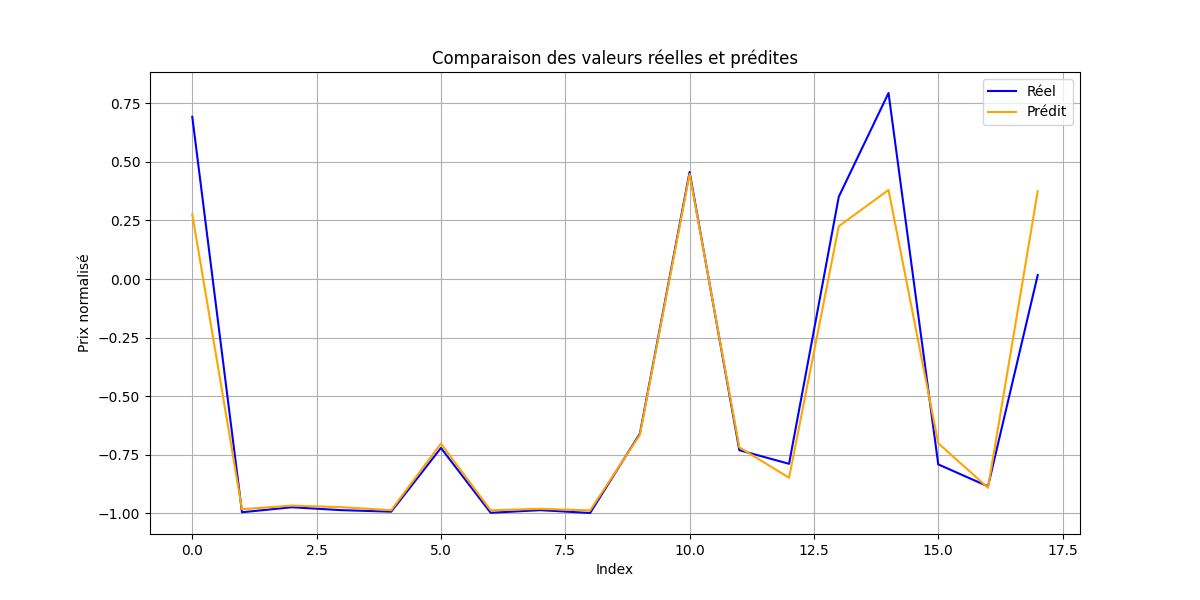
\includegraphics[width=0.8\textwidth]{img/Prediction.png}
    \caption{Real vs. Predicted Bitcoin Prices}
    \label{fig:predictions}
\end{figure}

\section{Conclusions and Perspectives}
\subsection{Summary of Findings}
The LSTM model developed in this project was able to predict Bitcoin prices with a reasonable degree of accuracy. The model captured the overall trend of Bitcoin prices, although there were some discrepancies between the predicted and actual prices.

\subsection{Future Work}
Future work could involve exploring different model architectures and hyperparameters to improve the prediction accuracy. Additionally, incorporating more features such as trading volume and market sentiment could potentially enhance the model's performance.

\section{Team Presentation}
\subsection{Chantoiseau Sacha}
Role: Data Preprocessing and Model Training

\subsection{Cherigui Allah Eddine}
Role: Model Evaluation and Results Visualization

\subsection{Louis Malmassary}
Role: Report Writing and Project Coordination

\end{document}
